\section{Optimize and Evaluate Alternatives}
\label{section:optimize-and-evaluate-alternatives}
\label{sec:framework-trade-review}

The independent review recommends PA-VS under a declared analyst reuse-first priority. This is a conditional design direction, with no procurement verdict, measured ranking or global optimum. OOSEM requires a common analysis context linked to stakeholder measures \citep[Secs.~8.11 and~17.3.6]{friedenthal2014practical}. Historical candidate values, scores and the Git/YAML winner are superseded.

\subsection{Common basis, gates and evidence}

Compare the complete minima, including all additions and dependencies, on the same cases, tasks, references and supported profiles. Pin models/solvers to isolate overhead, then assess native end-to-end work. Include manual steps, access, maintenance and recovery. Scenes earn credit only through activated decision-specific validation. CPU controller SIL and supplied-data replay remain required. HIL needs later equipment, timing and safety evidence.

Six noncompensable gates precede empirical ranking: EG-01 named coverage for every mandatory obligation, EG-02 semantic and correct-change integrity, EG-03 credible and safe limitation handling, EG-04 independent retained reconstruction, EG-05 frozen-core two-case reuse, and EG-06 legal/deployable access, versions, exports and recovery. All five concepts have compatible proposed realizations and unresolved checks. None has passed implementation gates. Critical findings block affected supported claims. Incorrect tasks receive no favorable burden credit.
{\small
\setlength{\tabcolsep}{4pt}
\setlength{\parskip}{0pt}
\setlength{\LTpre}{0.4\baselineskip}
\setlength{\LTpost}{0.4\baselineskip}
\renewcommand{\arraystretch}{1.06}
\begin{longtable}{@{}>{\raggedright\arraybackslash}p{\dimexpr0.55\linewidth-2.2\tabcolsep\relax}>{\raggedright\arraybackslash}p{\dimexpr0.16\linewidth-0.64\tabcolsep\relax}>{\raggedright\arraybackslash}p{\dimexpr0.29\linewidth-1.16\tabcolsep\relax}@{}}
\caption{Common trade dimensions. Numbers identify MN/MOE and FR.}\label{tab:framework-trade-criteria}\\
\toprule
\textbf{Criterion} & \textbf{MN/MOE} & \textbf{FR} \\
\midrule
\endfirsthead
\caption[]{Common trade dimensions. Numbers identify MN/MOE and FR. (continued).}\\
\toprule
\textbf{Criterion} & \textbf{MN/MOE} & \textbf{FR} \\
\midrule
\endhead
\bottomrule
\endfoot
DC-01 Guided requirements & 01 & 01--03, 17 \\
DC-02 Continuity/change & 02 & 04--09, 11 \\
DC-03 BOM/financial basis & 03 & 12--14 \\
DC-04 Dynamic EPS/disciplines & 04 & 15--19, 23, 24 \\
DC-05 Credibility/battery/diagnostics & 05 & 20--25 \\
DC-06 RAM & 06 & 26, 27 \\
DC-07 Safe proposals/observations & 07 & 28--32 \\
DC-08 Software/target resources & 08 & 33--36 \\
DC-09 Replay/readable justification & 09, 10 & 10, 37, 38 \\
DC-10 Adoption/lifecycle burden & 11 & 02, 10, 39, 40 \\
\end{longtable}
}

N means reported native service, D demonstrated source subset, T transferable mechanism, P project proposal and U unknown feasibility/benefit. These categories are not scores. All complete candidates include P additions and have U empirical MOE values. The full source-resolved ten-by-five matrix remains in the trade registry.
{\small
\setlength{\tabcolsep}{4pt}
\setlength{\parskip}{0pt}
\setlength{\LTpre}{0.4\baselineskip}
\setlength{\LTpost}{0.4\baselineskip}
\renewcommand{\arraystretch}{1.06}
\begin{longtable}{@{}>{\raggedright\arraybackslash}p{\dimexpr0.15\linewidth-0.6\tabcolsep\relax}>{\raggedright\arraybackslash}p{\dimexpr0.43\linewidth-1.72\tabcolsep\relax}>{\raggedright\arraybackslash}p{\dimexpr0.42\linewidth-1.68\tabcolsep\relax}@{}}
\caption{Evidence leverage and decisive uncertainty on the same minimum scope.}\label{tab:framework-trade-evidence}\\
\toprule
\textbf{Candidate} & \textbf{Scoped leverage} & \textbf{Open burden} \\
\midrule
\endfirsthead
\caption[]{Evidence leverage and decisive uncertainty on the same minimum scope. (continued).}\\
\toprule
\textbf{Candidate} & \textbf{Scoped leverage} & \textbf{Open burden} \\
\midrule
\endhead
\bottomrule
\endfoot
PA-COM & N/D catalogue, ownership, categorical budgets and tutorial (COM-E04--08). & P rich semantics/releases and expanded domain assurance. U current API and Excel replay. \\
PA-CDT & T CSRM and partial native assets (E01/E04). P local semantic CPU authority. & P guidance, quantities/change logic, FMI, RAM and profiles. Optional scenes add separate clocks/licenses. \\
PA-GY & D versioned text, documents, alternatives and packet definitions (GY-E05--09). & P complete schemas/integrations. Source limits include stale content and participation (E11). \\
PA-NS & N/D collaboration, extraction, dependency graphs and budgets (NS-E01/E08--10). & P model/graph/release reconciliation and off-nominal/domain assurance. U maintained stack. \\
PA-VS & N requirements/value/procedure surfaces. D tree/mode/budget transfers (VS-E01--07/E09). & P stable-ID recovery, replay and domain assurance. U access/exports and synchronization burden. \\
\end{longtable}
}

Mode values establish no coupled dynamics. The OpenModelica EPS demonstration was a separate ENOVIA/SIMULIA workflow \citep[Sec.~4.4]{review-0793}. It is transferable evidence. Native Tests records establish no technician-safe procedure.

\subsection{Selection and reversal conditions}

The priority favors reuse of documented requirement, architecture, engineering-value and procedure services before recreating general services. PA-VS has the strongest combined source basis for that priority \citep[Secs.~2.1 and~3.3--3.4]{citation-4690}\citep[Secs.~3.1 and~4.3--4.4]{campioli2025integration}. This addresses expanded manager, systems and technician concerns. It proves no lower total effort, cost or error rate. Complete model, RAM, software, safety and replay services remain substantial development.

Reopen selection if access/export/recovery fails, stable-ID transactions fail, or synchronization removes reuse benefit. PA-CDT's CPU core is the principal alternative under local semantic authority and portable release priorities, conditional on its native quantity, FMI and replay checks. The other three remain admissible if complete common-task evidence supports them. First compare requirement/procedure work, a coupled subsystem/BOM/software change and clean replay after working-data changes. Continue all V and MOE protocols. Raw outcomes/uncertainty precede Pareto or utilities. The empirical Pareto set is undetermined. Any later score needs explicit preferences, anchors and sensitivity. Avoid double counting. Literature frequencies and evidence categories give no cardinal weights.

\subsection{Selected physical scope and component obligations}
\label{section:selected-physical-architecture}

The four PA-VS partitions may share hosts. Generic libraries, adapters and methods are framework assets. Mission-specific models, hardware and software designs are controlled case artifacts.

\begin{figure}[!htbp]
\centering
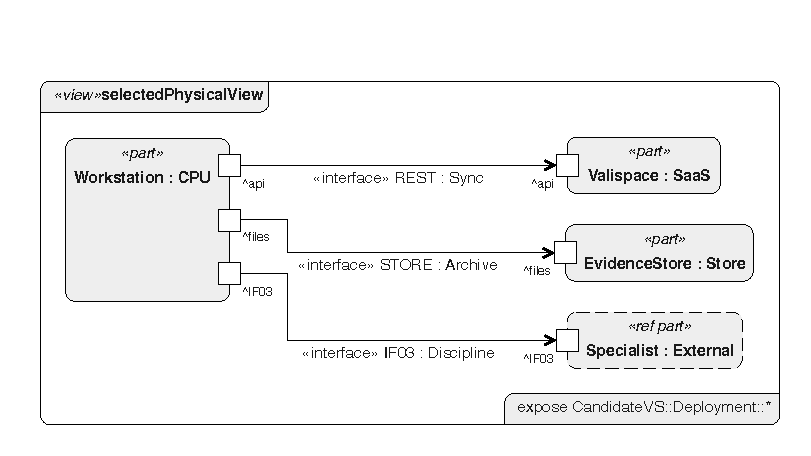
\includegraphics[width=\linewidth]{figures/sysml/physical/sysml-defined-view-reportviews-selectedphysicalview.pdf}
\caption{Proposed PA-VS deployment. The workstation, hosted engineering service and controlled store realize the four responsibility partitions. The specialist node is external. Host roles may share equipment. Access and reconstruction remain to be verified.}
\label{fig:framework-physical}
\end{figure}

Table~\ref{tab:selected-framework-allocation} names the reviewed bounded modules/data profiles. All additions are proposed. The registry retains their full forty FR allocations, procedures, hosts and maturity.
{\small
\setlength{\tabcolsep}{4pt}
\setlength{\parskip}{0pt}
\setlength{\LTpre}{0.4\baselineskip}
\setlength{\LTpost}{0.4\baselineskip}
\renewcommand{\arraystretch}{1.06}
\begin{longtable}{@{}>{\raggedright\arraybackslash}p{\dimexpr0.26\linewidth-1.04\tabcolsep\relax}>{\raggedright\arraybackslash}p{\dimexpr0.34\linewidth-1.36\tabcolsep\relax}>{\raggedright\arraybackslash}p{\dimexpr0.4\linewidth-1.6\tabcolsep\relax}@{}}
\caption{Selected component obligations and primary allocations. FR numbers and VS-PC- component suffixes are shown.}\label{tab:selected-framework-allocation}\\
\toprule
\textbf{L / primary FR} & \textbf{Physical realizations} & \textbf{Component obligation} \\
\midrule
\endfirsthead
\caption[]{Selected component obligations and primary allocations. FR numbers and VS-PC- component suffixes are shown. (continued).}\\
\toprule
\textbf{L / primary FR} & \textbf{Physical realizations} & \textbf{Component obligation} \\
\midrule
\endhead
\bottomrule
\endfoot
L01 / 02, 03 & GUIDANCE, PROCEDURES, EVALUATION, WEB & Sourced methods, qualitative/quantitative examples and learning records. \\
L02 / 01, 04--06, 11, 17, 26 & GOVERNANCE, WEB, CASE, BRIDGE & Requirement/decision schemas, typed relation index, impacts and stale/claim status. \\
L03 / 15, 18, 33--36 & CAPELLA, EPS-TEMPLATE, FSW, CONTRACT & Topology/modes, reusable structure, detailed dictionaries and both checked target profiles. \\
L04 / 12, 13, 27 & CHARACTERIZATION, WEB, CASE, RAM & Sourced components, BOM/quotes/failures and Capella-to-FMEA transformation. \\
L05 / 10, 14, 16, 19, 20, 23, 24 & SCENARIO, EPS-ENGINE, RUNNER, RAM, FSW, ARCHIVE & Frozen time histories/settings, virtual controller/policy cases and proposed integrated OpenModelica. \\
L06 / 21, 22, 25, 31, 32 & CREDIBILITY, OBSERVATION, MODELS, EVIDENCE & Fit/validation/applicability, updates/residuals and raw channel/clock/validity checks. \\
L07 / 28--30 & VERIFICATION, WEB, PROCEDURES, EVIDENCE & Method-specific Tests templates, technician export and completeness/readiness gates. \\
L08 / 07--09 & CONTRACT, BRIDGE, ARCHIVE, EVIDENCE & IDs/semantics, reviewed diff/recovery, composite baselines and raw custody. \\
L09 / 37--40 & WEB, REVIEW, EVALUATION, CASE, ARCHIVE & Controlled views/feedback, installation/tasks and frozen-core case evaluation. \\
\end{longtable}
}

Capella owns topology, allocation and transitions. Valispace owns requirement text, criterion references, characteristics, quantities, quotes and formulas. FSW owns detailed service semantics. Generated views reference these sources. MODELS owns analysis, calibration, validity and controller revisions. ARCHIVE/EVIDENCE retains released manifests and raw outputs. BRIDGE requires stable IDs, dry-run diffs, reviewed application and recovery for rename, deletion, conflicting/interrupted updates. Name-only repair is insufficient. Aging/controller adequacy remains case-model development.

VS-HOST-ENG executes Capella and its internal Python scripts. It also executes the bridge, domain modules and proposed OpenModelica. VS-HOST-VALI supplies vendor execution/storage. VS-HOST-STORE retains managed evidence with backup arrangements to confirm. VS-HOST-SPECIALIST and VS-HOST-FLIGHTBUILD are external controlled discipline/build services. Profiles must pin versions, mappings and access. No GPU, replica or real-time target is mandatory. SE stewards requirements/releases, EPS/PM components/costs, qualified contributors models/software, and EPS/technician proposals with external facility authority. Start with the reported in-application path \citep[Sec.~3.3]{citation-4690}. Headless export is a separately verified option. Rights, sizing and model data remain unresolved.
